\chapter{水下图像合成实验与分析评测}
本章将针对水下图像多模态转译问题设计实验、确定评价指标,验证我们设计的网络模块的有效性,并与基准方法进行对比和分析。

\section{水下图像多模态合成实验设计}
\subsection{实验设置}
基准方法我们总共选取了五种,其中两种经典的图像转译方法CycleGAN~\citep{zhu2017unpaired}和基于分解表示的跨域多模态转译方法MUNIT~\citep{huang2018multimodal},三种最新的图像多模态转译方法DRIT++~\citep{lee2020drit++}、DSMAP~\citep{chang2020domain}和StarGAN v2~\cite{choi2020stargan}。除了不可或缺的经典模型CycleGAN,剩余四种方法都可以完成两个域之间的多模态转译任务。

CycleGAN学习两个域之间的一对一映射,通过循环一致性损失能够很好的学习到目标域的特征;MUNIT, DRIT++ and DSMAP将图像分解为共享的内容空间和不同域的特征空间,然后通过给生成器共享的内容和目标域的特征合成目标域风格相同内容信息的结果;StarGAN v2使用一个生成器结构,通过编码控制生成具有多个特征的多个目标域。所有基准方法的训练代码均来自作者Github提供完成版本。

在我们的实验室中,将$A$域设置为空中域,$B$域设置为多模态水下域,在以上五种基准方法上进行多个数据集的客观实验。在真实水下数据集和合成数据集上设置了针对模糊程度、水颜色、以及特定水质状态的多个实验。

\subsection{数据集设置}
由于水下环境导致采集数据限制,我们的数据集并不是十分充足,因此在一种实验实验设置中用到多个数据集的组合结果。我们在水下图像多模态转译任务中,主要使用到RUIE~\citep{liu2019real}, UWCNN~\citep{li2020underwater}, UVB 2017数据集。EUVP~\citep{islam2019fast}和UIEB~\citep{li2019underwater}数据集就作为补充进行组合实验。其中RUIE,UIEB和EUVP部分数据集是真实世界水下图像结果,UWCNN和UVB 2017是合成图像结果。这些数据集在各个子集数量上并不都是均衡的,所以训练时对模型方法提出了较高的要求。

RUIE数据集是一个真实世界获取到的水下不配对图像集。当我们进行水下色偏和清晰度实验训练时,选择RUIE的子集UCCS的300张图片当作水下域,选取EUVP中300张无水子集作为空中域。进行测试实验时,选择EUVP中的100张无水图像作为空中域,测试训练模型,以获得水下多模态域的结果。

UWCNN数据集使用NYU-v2的RGB-D图像来合成深海和近海的十种水类型。基于水下衰减模型,多个衰减系数当作不同的水类型的控制变量。当我们进行训练时,选择1200张衰减系数为0即无水域,选择近海type-1,type-3,type-5,type-7作为水下多模态域,每种类型选取300张,这几种水下类型在视觉上有直观可见的区别,方便后续进行定性评价。进行测试时,选择无水域中249张进行测试。

Underwater Vision Benchmark 2017 (UVB 2017)是我们实验室用ZED和Kinect立体摄像机捕获的图像和视频数据集。在大连进行了模拟浑浊度实验,将不同浓度的\ce{Al(OH)3}模拟不同水质类型的浑浊度,相机收集相同目标物在不同距离和不同水质下的多种结果。训练时,我们选择了66张作为无水域,447张不同深度和浑浊度的结果作为水下多模态域。测试时,无水域选取66张进行测试。

\subsection{评价准则}
为了方便对各个方法进行客观对比,在图像转译角度从转译结果真实性、多样性来进行评价。

\textbf{真实性。}真实性是指给定源域$x_A$图像作为输入,生成的结果应该域目标域$x_B$中的分布尽可能的相同。在我们实验中,生成的水下多模态域的结果应该在质量真实性评价上尽可能的相近。

我们在实验中,真实性指标选取Fréchet Inception Distance(FID)来进行评价。基于Inception score改进,FID最初由Heusel等人~\cite{heusel2017gans}提出。FID能够完善Inception score没有比较模型生成样本和真实样本统计特性的问题。真实图像假设它是服从一个高斯分布,生成样本的分布应该与真实样本的分布尽量相同。这两个n维
变量分布之间的距离用Wasserstein-2 distance或者叫Fréchet distance来进行计算,较低的FID意味着两个分布之间更接近,也就意味着生成图片的跟真实结果之间相似性较高。

\textbf{多样性。}非成对图像多模态转译问题中,在输入唯一时,能产生目标域的多模态结果。在我们到水下图像多模态转译任务中,在输入一张空中图像时,我们希望能得到多个对应的水下域图像转译结果。即使都是相同的内容,在水质等水下条件不同导致水下图像的模态不一致。对于生成的多种图像,都能跟输入图像拥有相同的内容,再对生成结果进行多样性的评价。

在实验中,我们选用Learned Perceptual Image Patch Similarity (LPIPS)来评价多样性指标。LPIPS最初由Zhang等人~\cite{zhang2018perceptual}提出,用于衡量成对图像之间的相似程度。相比于传统的图像相似度评价指标,LPIPS指标得到的结果和人的视觉评价有更高的相关性。对于多对图像,排列组合成平方次图像对,计算每对之间的相似性,求得平均值作为指标的结果。

\section{水下图像多模态合成结果分析}
\subsection{定性结果分析}

\begin{figure*}[htp]
    \centering
	\includegraphics[width=\textwidth]{figures/RUIE_random_1.pdf}
	\caption{在RUIE数据集上,基准方法和我们提出的方法在目标域随机采样生成的多模态结果比较。}
	\label{fig:ruie_random_1}
\end{figure*}

\begin{figure*}[htp]
    \centering
	\includegraphics[width=\textwidth]{figures/RUIE_random_2.pdf}
	\caption{在RUIE数据集上,基准方法和我们提出的方法在目标域随机采样生成的多模态结果比较。}
	\label{fig:ruie_random_2}
\end{figure*}

\begin{figure*}[htp]
    \centering
	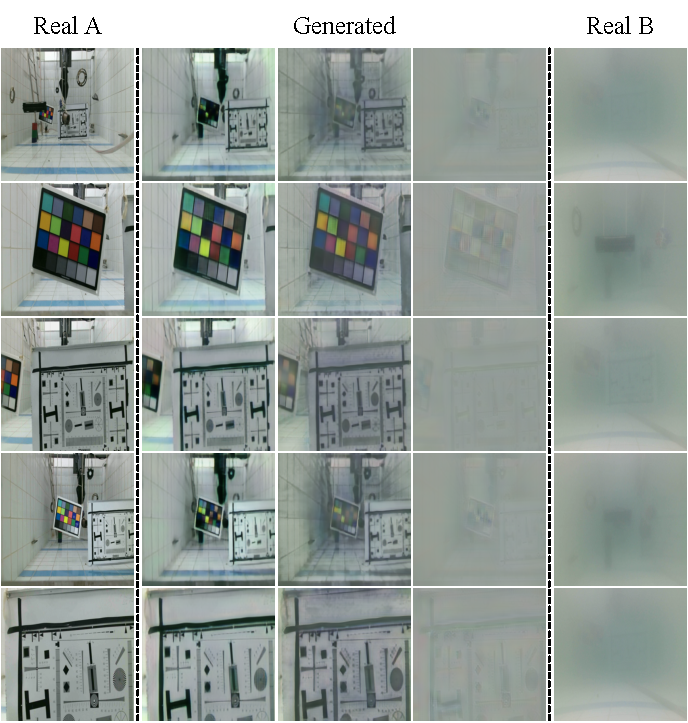
\includegraphics[width=\textwidth]{figures/UVB_random.pdf}
	\caption{在UVB数据集上,基准方法和我们提出的方法在目标域随机采样生成的多模态结果比较。}
	\label{fig:uvb_random}
\end{figure*}

\begin{figure*}[htp]
    \centering
	\includegraphics[width=\textwidth]{figures/UWCNN_random.pdf}
	\caption{在UWCNN数据集上,基准方法和我们提出的方法在目标域随机采样生成的多模态结果比较。}
	\label{fig:uwcnn_random}
\end{figure*}

\begin{figure*}[ht]
    \centering
	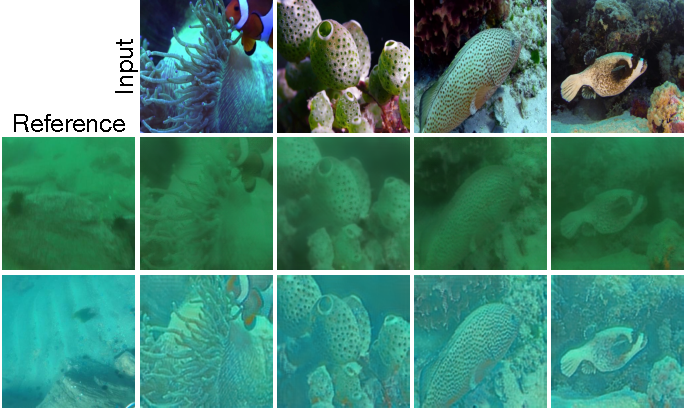
\includegraphics[width=\textwidth]{figures/RUIE_guidance.pdf}
	\caption{tongg}
	\label{fig:ruie_guide}
\end{figure*}

\begin{figure*}[ht]
    \centering
	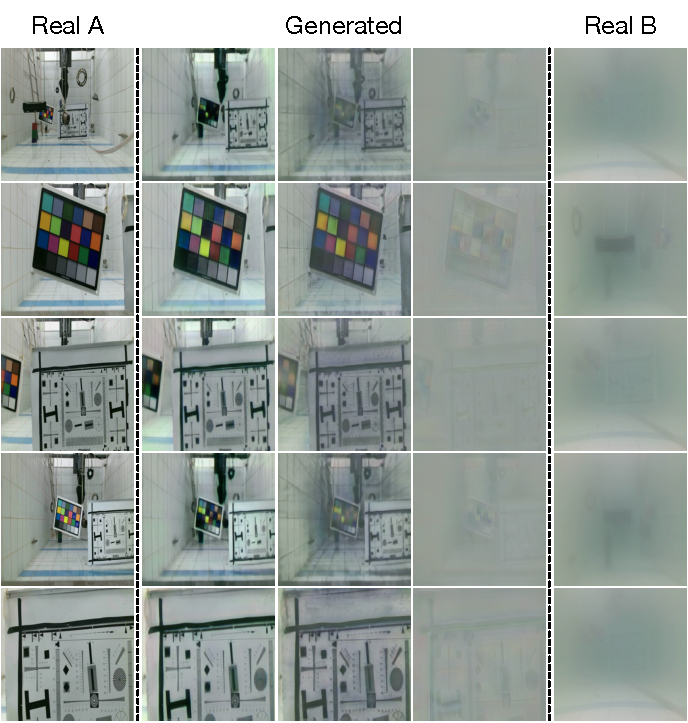
\includegraphics[width=\textwidth]{figures/UVB-change.pdf}
	\caption{tongg}
	\label{fig:uvb-change}
\end{figure*}

图~\ref{fig:ruie_random_1}和图~\ref{fig:ruie_random_2}展示了不同方法在RUIE数据集上的定性结果对比。从对比图中可以看到,CycleGAN+noise方法的转译结果比较真实,内容信息保留完整,但是噪声被忽略,不同风格采样信息加入的每行没有多模态样式的结果;MUNIT方法转译结果质量较差,内容丢失了大量的信息,内容轮廓信息几乎全部丢失,尽管模态之间能看出区别,从行结果上看同样的风格采样信息影响的风格样式并没有一致;DSMAP方法中每行风格信息影响的样式上能看出一致的差异,很明显内容和风格也没有分解彻底,DSMAP每行的

\subsection{定量结果分析}

\begin{table*}[ht]
\centering
\caption{在RUIE、UWCNN、UVB 2017数据集上的真实性和多样性定量比较。}
\begin{tabular}{|p{2.5cm}|p{1.7cm}|p{1.7cm}|p{1.7cm}|p{1.7cm}|p{1.7cm}|p{1.7cm}|}
\hline
\multirow{2}{*}{Methods} & \multicolumn{2}{c|}{RUIE} & \multicolumn{2}{c|}{UWCNN} & \multicolumn{2}{c|}{UVB 2017} \\ \cline{2-7} 
                         & FID           & LPIPS       & FID           & LPIPS          & FID            & LPIPS          \\ \hline \hline
CycleGAN                 & 243.4         & 0.634       & \textbf{80.7} & 0.490          & \textbf{145.1} & 0.358          \\ \hline
MUNIT                    & 139.4         & 0.452       & 232.1         & 0.647          & 240.4          & 0.486          \\ \hline
DRIT++                   & 179.2         & 0.575       & 290.7         & 0.668          & 243.7          & 0.474          \\ \hline
DSMAP                    & 139.6         & 0.513       & 138.8         & 0.513          & 232.6          & 0.344          \\ \hline
StarGAN v2               & 121.1         & 0.431       & 162.8         & 0.358          & 129.8          & 0.595          \\ \hline
Ours                     & \textbf{83.2} & \textbf{0.579} & 149.6      & \textbf{0.732} & 172.7          & \textbf{0.493} \\ \hline
\end{tabular}
\label{tab:modal_compare}
\end{table*}

真实性和多样性定量指标如表~\ref{tab:modal_compare}
在真实水下获取到的RUIE数据集上,CycleGAN、MUNIT、DRIT++、DSMAP

DSMAP工作基于MUNIT工作进行的改进,

\subsection{消融实验}

\section{水下图像多样式域合成实验设计}
\subsection{实验设置}

\subsection{数据集设置}

\subsection{评价准则}

\section{水下图像多样式域合成结果分析}
\subsection{定性结果分析}

\subsection{定量结果分析}


\subsection{消融实验}
